\chapter{Interfaccia web di configurazione}\label{capitolo5}
In questo capitolo vengono esposti la progettazione e l'implementazione dell'interfaccia web di configurazione
nel MM.
Al fine di ospitare la pagina web che contiene il pannello di configurazione, \`e necessario
creare una nuova classe server oltre a quella gi\`a esistente, citata nel sezione \ref{cap:MMalto}.
Il server gira su una porta differente rispetto al primo server, la quale è indicata nel file di configurazione del MM,
ed \`e accessibile da qualsiasi utente all'interno della sottorete.
La struttura del server viene gestita con Express, spiegato nella sezione \ref{cap:express}, che offre funzioni per gestire
pi\`u facilmente le richieste delle pagine e le relative risposte.
Inoltre, all'inizializzazione del server, viene passato come parametro il file di configurazione del
MM.\\
Affinch\`e l'interfaccia funzioni completamente \`e stato necessario inserire una nuova dipendenza:
per ogni modulo deve essere creato un file JSON con lo stesso nome,
contenente i campi e le variabili della propria configurazione.\\
In particolare, nel capitolo, verranno esposte la struttura del funzionamento dell'interfaccia (sezione \ref{cap:strutturainterfaccia}) e le metodologie per
l'individuazione dei moduli
presenti nel MM, con i relativi file JSON, al fine di renderli modificabili (sezione \ref{cap:individuazione}).\\[1\baselineskip]

\section{Struttura dell'interfaccia Web di configurazione}\label{cap:strutturainterfaccia}
Dato che il server \`e implementato con Express, la struttura
\`e caratterizzata dalle due entit\`a (Controller e Modello), descritte nella sezione \ref{cap:express}.
Come mostrato in figura \ref{fig:struttinterfaccia},
un utente (tramite il browser) fa richiesta di una pagina di un determinato modulo passando un Uniform Resource Identifier(\textit{URI}),
che viene ricevuto dal controller principale (passo 1) e inoltrato al modello (passo 2) a cui fa riferimento (in questo caso il modello
\`e uno soltanto). Il modello ricerca in locale il file JSON del modulo richiesto (passo 3) e lo passa al controller (passo 4 e 5), il quale lo
inoltra alla vista.
Quest'ultima aggiorna il template della pagina inserendo i dati contenuti nel JSON che \`e stato passato, e la inoltra al browser che ne ha fatto richiesta.\\
Non \`e stato necessario utilizzare il Routing dal momento che \`e stato necessario
implementare un solo modello e, di conseguenza, un solo controller.\\[1\baselineskip]

\begin{figure}[H]
    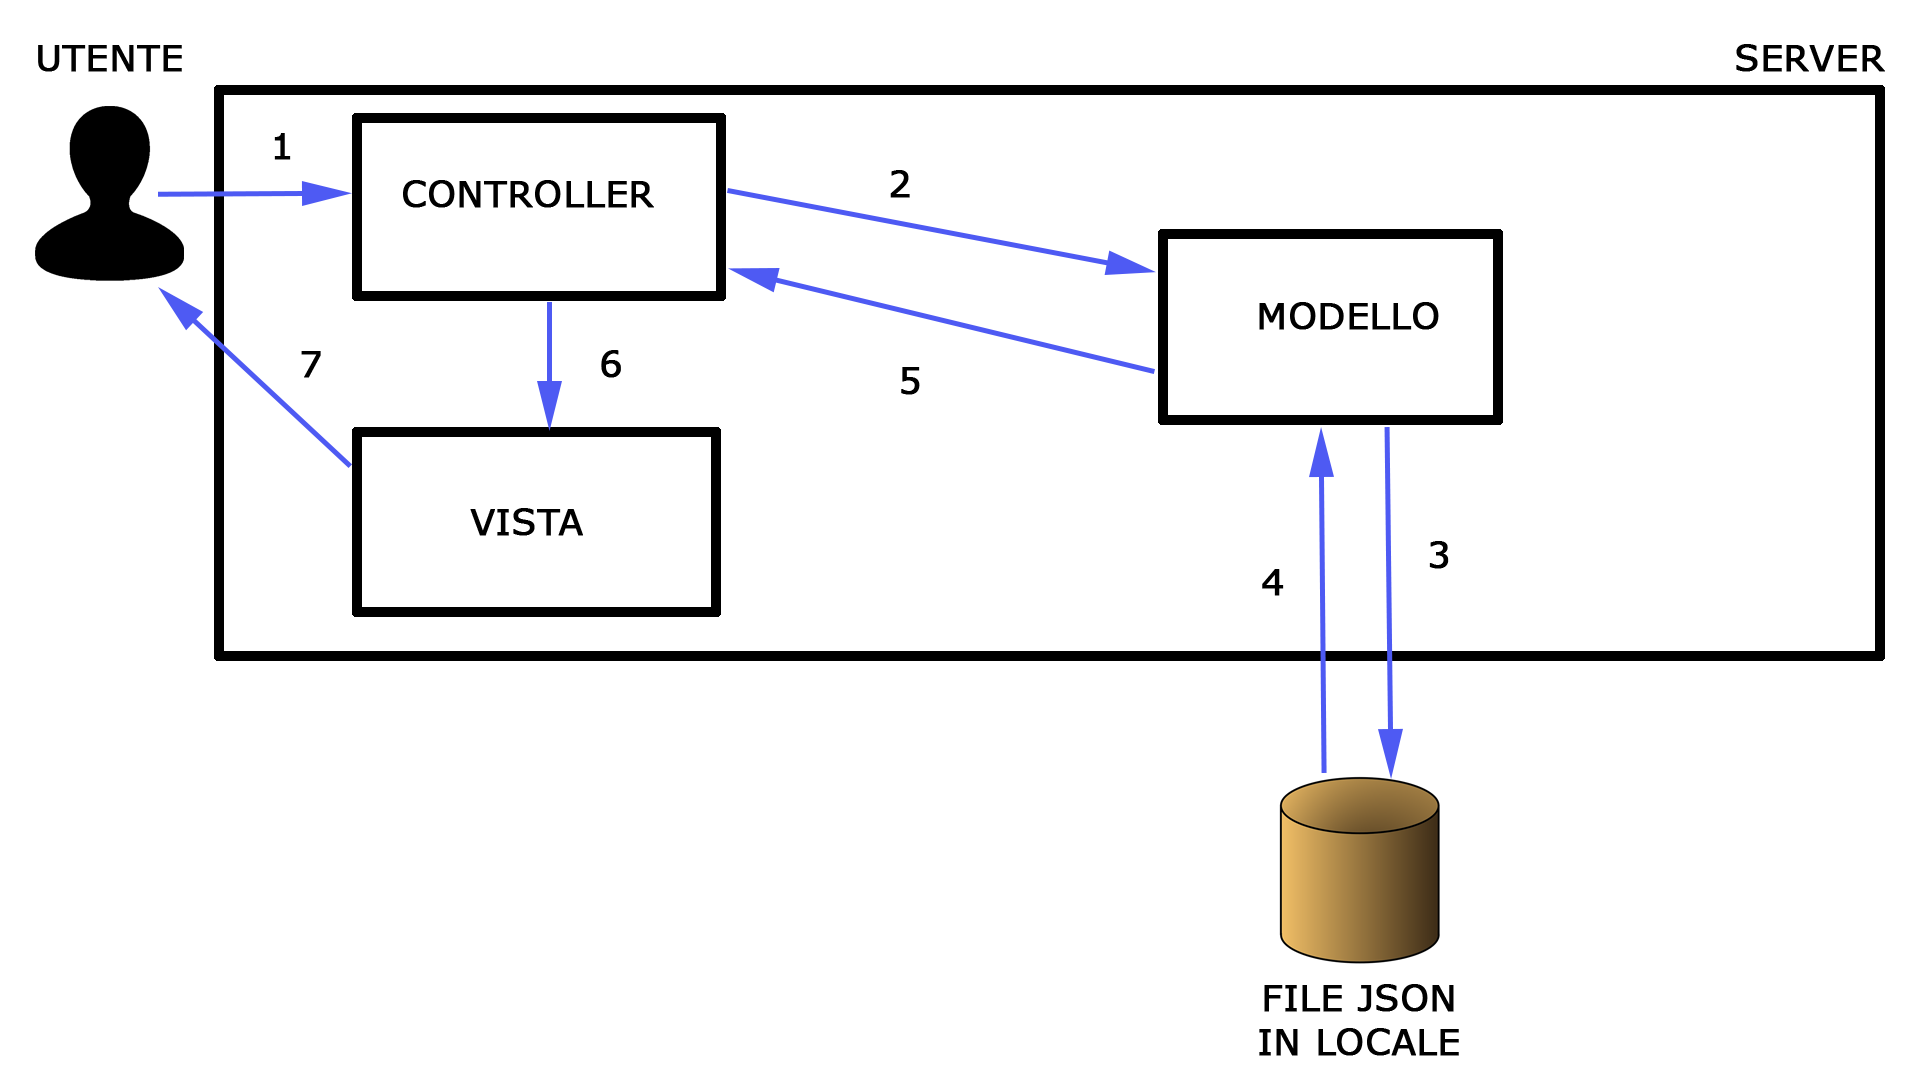
\includegraphics[width=1\textwidth, height=0.4\textheight]{interfacciatesi}
    \caption{Struttura del server dell'interfaccia web}
    \label{fig:struttinterfaccia}
\end{figure}

\section{Individuazione e visualizzazione dei moduli nell'interfaccia}\label{cap:individuazione}
Come gi\`a discusso nella sezione \ref{cap:app}, tutti i moduli sono contenuti nella
cartella \textit{Modules} del MM. Il server, tramite una funzione della libreria,
legge i nomi di tutte le cartelle contenute all'interno di \textit{Modules}, il cui percorso \`e stato passato
come parametro alla funzione. In seguito, salva tutti i nomi dei moduli
in una lista, filtrando i file e le cartelle che non si riferiscono ad essi.
La funzione per leggere le directory, appena citata, offre un metodo per leggere ed elencare le cartelle in
modo sincrono, cos\`i da non rendere necessario l'utilizzo di callback.\\
All'interno di \textit{Modules} \`e presente una cartella \textit{default}, che contiene
i moduli standard in dotazione con il MM. Per poter elencare anche questi ultimi \`e stato necessario utilizzare la funzione
di libreria precedentemente usata anche su quest'ultima cartella e concatenare, successivamente, le due liste,
per ottenere un'unica lista con tutti i moduli, necessaria per poter popolare il men\`u del pannello web di configurazione.\\
Tutte le pagine web che ritorna il server sono divise in 2 sezioni come illustrato nella figura \ref{fig:interfaccia}:
\begin{itemize}
\item Il men\`u laterale, che contiene tutti i moduli messi nella lista (ad esempio \textit{calendar} e \textit{clock}). Ogni opzione del men\`u corrisponde ad un modulo, che inoltra
la richiesta con il rispettivo URI
\item Le varie impostazioni del modulo, visualizzate tramite \textit{CodeMirror}\cite{CodeMirror}, una componente Javascript
che permette l'implementazione di un'area di testo per la modifica di codici all'interno di una pagina web.\\[1\baselineskip]
\end{itemize}
Una pagina web consiste in un file con estensione \textit{mustache} contenente
codici HTML e variabili Mustache, motore di template esposto nella sezione \ref{cap:mustache}.
Il server, alla richiesta di una pagina di uno specifico modulo, ricerca il relativo file JSON all'interno della cartella del modulo stesso e lo
passa come parametro sottoforma di oggetto JSON alla funzione \textit{render}, necessaria per la creazione e visualizzazione della pagina.
Insieme vengono passati i parametri \textit{posizione} ed \textit{header}, trattati nella sezione \ref{cap:MMconf}, estratti dal file
di configurazione passato all'inizializzazione del server.
Durante la creazione della pagina, i vari campi trasmessi, vengono inseriti dentro l'area di testo di \textit{CodeMirror}, che permetter\`a di eseguirne
le modifiche. Sotto all'area di testo \`e presente un bottone, che permette di attivare o disattivare il modulo nel MM; tuttavia affinch\`e la modifica
venga apportata \`e richiesto un riavvio manuale del software.
Le modifiche effettuate vengono spedite al server che si occupa di salvarle nel file di configurazione
principale del MM. Le metodologie e le pratiche per modificare e salvare le modifiche nel file di configurazione sono state sviluppate ed
implementate da una mia collega.\\
Nel caso che durante una delle operazioni di fetch o di invio dei dati alla pagina si verifichi un errore, viene mostrata una pagina
con un errore generico. Invece, in caso di errata sintassi del file JSON modificato, viene ricaricata la pagina del modulo appena modificato
mostrando una stringa di errore sopra all'area di editor di testo.


\begin{figure}[H]
    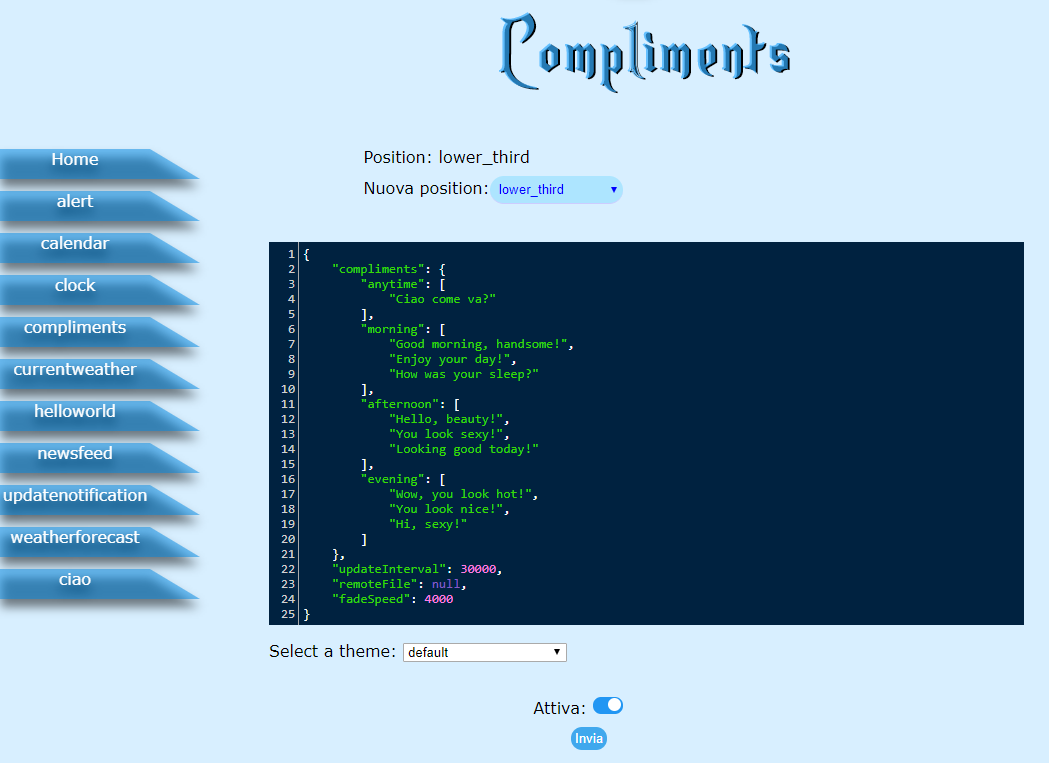
\includegraphics[width=1\textwidth, height=0.5\textheight]{interfacciamm}
    \caption{Interfaccia web di amminsitrazione}
    \label{fig:interfaccia}
\end{figure}
